\chapter{Satz von Fubini}
  \begin{remark}[Prinzip von Cavalieri]
    Haben zwei Körper in jeder Höhe Schnitte von gleichem Flächeninhalt, so haben sie auch auch das gleiche Volumen.    
  \end{remark}

  \begin{example}
    \begin{enumerate}
      \item Volumen eines Kegels.\\
        Sei $B \subseteq \mathbb{R}^2$ ein Gebiet mit Flächeninhalt $|B| = A$.\\
        Betrachte $C = \{s(b,1) \ | \ b \in B, 0 \leq s \leq 1\}$\\
        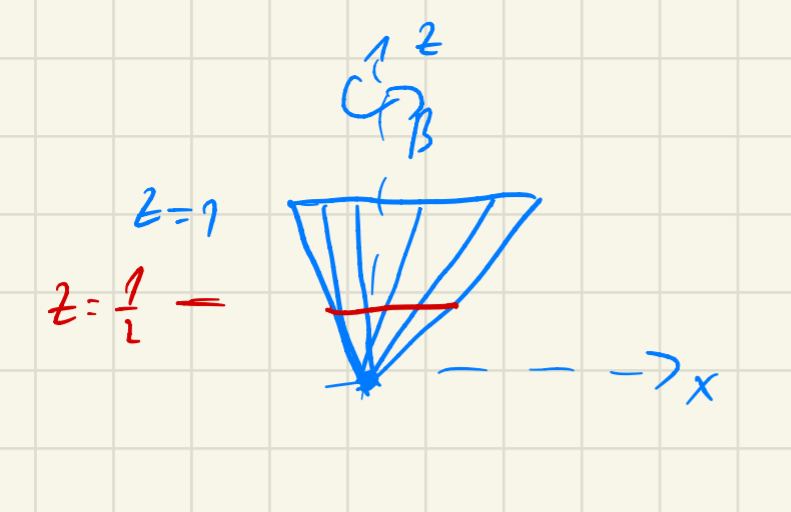
\includegraphics[width=3.5cm]{img/VI_Bsp_1_Kegel.png}\\
        Für $k \in [0,1]$ ist der $k$-Schnitt von $C$ die Menge \\
        $C_k = \{a \in \mathbb{R}^2 \ | \ (a,b) \in C\} = \{h \cdot b \ | \ b \in B\} = kB$\\
        $|C_k| = k^2A$ Nach Cavalieri hängt $vol(C)$ nur von $A$ ab.\\
        Wir schreiben $vol(C) = V(A)$. Es gilt $V(kA) = kV(A)$ für $k \in \mathbb{N}$, betrachte dazu ... (siehe Aufschrieb)
        \item Betrachte in $\mathbb{R}^3 = \mathbb{R}^2 \times \mathbb{R}$ die Mengen und die Inhalte der Zugehörigen $z$-Schnitte:
        \begin{align*}
          &\text{Zylinder } Z=\{(x,y,z) \ | \ \sqrt{x^2 + y^2} \leq 1, 0 \leq z \leq 1\}, |Z_z| = \pi\\
          &\text{Kegel } C=\{(x,y,z) \ | \ \sqrt{x^2 + y^2} \leq z, 0 \leq z \leq 1\}, |C_z| = \pi z^2\\
          &\text{Halbkugel } H=\{(x,y,z) \ | \ \sqrt{x^2 + y^2} \leq \sqrt{1-z^2}, 0 \leq z \leq 1\}, |H_z| = \pi (1-z^2)\\
        \end{align*}
        $\implies |Z_z| = |C_z| + |H_z| \stackrel{Cavalieri}{\implies} vol(H) = vol(Z) - vol(C) = \pi - \frac{\pi}{3} = \frac{2}{3} \pi$\\
        $\implies vol(C) : vol(H) : vol(Z) = 1 : 2 : 3$ (Archimedes)
    \end{enumerate}
  \end{example}

  \begin{definition}
    Seien $\alpha, \beta$ äußere Maße auf $X,Y$. Das \textbf{Produktmaß} $\alpha \times \beta$ einer Menge $E \subseteq X \times Y$ ist
    \begin{align*}
      (\star) \ \ \alpha \times \beta (E) = inf\{\sum\limits_{j=1}^{\infty} \alpha(A_j) \beta(B_j) \ | \ A_j, B_j \text{ messbar}, E \subseteq \bigcup\limits_{j=1}^{\infty} A_j \times B_j\}
    \end{align*}
  \end{definition}

  \begin{lemma}
    $\alpha \times \beta$ ist ein äußeres Maß
  \end{lemma}
  \begin{proof}
    siehe Aufschrieb
  \end{proof}

  \begin{lemma}
    Sei $P = A \times B$. Eine Produktmenge, d.h. $A,B$ sind messbar bzgl. $\alpha$ bzw. $\beta$. Dann gilt $\alpha \times \beta(P) = \alpha(A) \beta(B)$ und $P$ ist $\alpha \times \beta$-messbar.
  \end{lemma}
  \begin{proof}
    siehe Aufschrieb
  \end{proof}

  \begin{theorem}[Cavalierisches Prinzip]
    Seien $\alpha$ und $\beta$ $\sigma$-endliche äußere Maße auf $X$ bzw. $Y$, und $D \subseteq X \times Y$ sei $\alpha \times \beta$-messbar. Dann ist $D_y = \{x \in X \ | \ (x,y) \in D\}$ $\alpha$-messbar für $\beta$-fast alle $y \in Y$. Die Funktion $y \mapsto \alpha(D_y)$ ist $\beta$-messbar und es gilt:
    \begin{align*}
      (\alpha \times \beta)(D) = \int\limits_Y \alpha(D_y) \ d\beta(y)
    \end{align*}
  \end{theorem}
  \sidenote{Vorlesung 17}{11.01.21}
  \begin{proof}
    siehe Aufschrieb
  \end{proof}

  \begin{remark}
    Die Rollen von $\alpha$ und $\beta$ können vertauscht werden, d.h. man betrachtet das $\beta$-Maß des $X$-Schnittes $D_x 0 \{y \in Y \ | \ (x,y) \in D\}$ und integriert bzgl. $\alpha$
    \begin{align*}
      \implies \alpha \times \beta (D) = \int\limits_Y \alpha(D_y) \ d\beta(y) = \int\limits_X \beta(D_x) \ d\alpha(x)
    \end{align*}
  \end{remark}

  \begin{example}
    Man kann nicht auf die $\sigma$-Endlichkeit verzichten.
    \begin{align*}
      D := \{(x,y) \in [0,1] \times [0,1] \ | \ x=y\} \subseteq \mathbb{R} \times [0,1]\\
      \int\limits_{\mathbb{R}} card(D_x) d\lambda^1(x) = 1 \neq 0 = \int\limits_{[0,1]} \lambda^1(D_y) \ d card(y)
    \end{align*}
    Mit $I_k = [\frac{k-1}{n}, \frac{k}{n}]$ gilt $D = \bigcap\limits_{n=1}^{\infty}( \bigcup\limits_{k=1}^{\infty} I_k \times I_k) \implies D$ ist messbar bzgl. $\lambda^1 \times card$
  \end{example}

  \newpage
  \begin{lemma}
    Es gilt $\lambda^n = \lambda^k \times \lambda^m$ für $k + m = n$
  \end{lemma}
  \begin{proof}
    siehe Aufschrieb
  \end{proof}

  \sidenote{Vorlesung 18}{15.01.21}
  \begin{example}
    \begin{enumerate}
      \item[]
      \item Volumen $\alpha_n$ der Kugel $B=\{z \in \mathbb{R}^n \ | \ ||z|| < 1\}.$\\
        Für $y \in [-1,1)$ ist $B_y = \{x \in \mathbb{R}^{n-1} \ | \ ||x|| < |1-y^2|^{1/2}\}$\\
        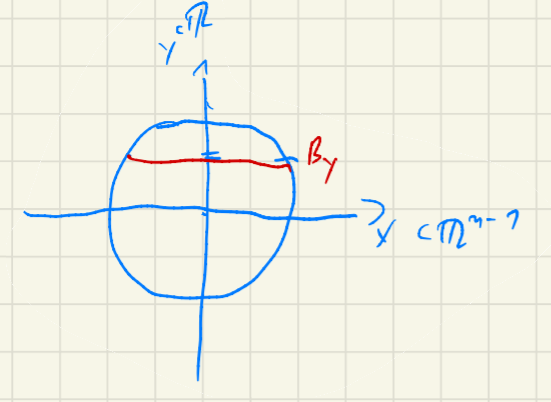
\includegraphics[width=3.5cm]{img/VI_Bsp_3_Kreis.png}
        \begin{align*}
          \alpha_n &=  \int\limits_{-1}^1 \lambda^{n-1}(B_y) \ dy = \alpha_{n-1} \int\limits_{-1}^1 (1-y^2)^{\frac{n-1}{n}} \ dy\\
          &\stackrel{y=\cos \theta}{=} \alpha_{n-1} A_n \text{, mit } A_n = \int\limits_0^{\pi} \sin^n\theta \ d\theta\\
          &\stackrel{part. Int.}{\implies} A_n = \frac{n-1}{n} A_{n-2} \ \forall \ n \geq 2 \text{, dabei sind } A_0 = \pi, A_1 = 2\\
          \implies A_{2k} &= \frac{2k-1}{2k} \cdot ... \cdot \frac{1}{2} A_0 = \pi \prod\limits_{j=1}^k \frac{2j}{2j+1}\\
          A_{2k+1} &= \frac{2k}{2k+1} \cdot ... \cdot \frac{2}{3} A_1 =2 \prod\limits_{j=1}^k \frac{2j}{2j+1}\\
          \implies A_{2k+1} A_{2k} &= \frac{2\pi}{2k+1} \text{ bzw. } A_{2k} A_{2k-1} = \frac{\pi}{k}\\
          \implies \alpha_{2k} &= (A_{2k}A_{2k-1}) ... (A_3 A_2) \alpha_0 = \frac{\pi^k}{k!}\\
          \alpha_{2k+1} &= (A_{2k}A_{2k-1}) ... (A_3 A_2) \alpha_1 = \frac{\pi^k}{(k+\frac{1}{2})(k-\frac{1}{2})...\frac{1}{2}}
        \end{align*}
        Bem: $\alpha_k \to 0$ mit $k \to \infty$
      \item Für $A \subseteq \mathbb{R}^n$ sei $K(A) = \{y (x,1) \in \mathbb{R}^n \times \mathbb{R} = \mathbb{R}^{n-1} \ | \ 0<y<1, x\in A\}$\\
        Beh: $A$ messbar bzgl. $\lambda^n$ $\implies$ $K(A)$ $\lambda^{n+1}$-messbar und $\lambda^{n+1}(K(A)) = \frac{1}{n+1}\lambda^n(A)$\\
        (siehe Aufschrieb)
    \end{enumerate}
  \end{example}

  \begin{definition}
    Eine Funktion $f: X \to [-\infty, \infty]$ heißt $\bm{\sigma}$\textbf{-endlich} bzgl. des äußeren Maßes $\mu$, falls gilt:
    $$f \text{ ist } \mu \text{-messbar und } \{f \neq 0\} \text{ ist } \sigma \text{-endlich}$$
  \end{definition}

  \begin{theorem}[Fubini]
    Seien $\alpha, \beta$ äußere Maße auf $X$ bzw. $Y$ und $f: X \times Y \to \bar{\mathbb{R}}$ sei $\sigma$-endlich bzgl. $\alpha \times \beta$. Ist das Integral $\int f \ d(\alpha \times \beta)$ definiert, so gilt:
    \begin{enumerate}
      \item Für $\beta$-fast alle $y \in Y$ ist $f(\cdot, y) \alpha$-messbar, und $\int\limits_X f(x,y) \ d \alpha(x)$ existiert.
      \item $y \mapsto \int\limits_X f(x,y) \ d\alpha(x)$ ist $\beta$-messbar und $\int\limits_Y \int\limits_X f(x,y) \ d\alpha(x) \ d\beta(y)$ existiert.
      \item $\int\limits_{X\times Y} f \ d(\alpha \times \beta) = \int\limits_Y \int\limits_X f(x,y) \ d\alpha(x) \ d\beta(y)$
    \end{enumerate}
    Der Satz gilt auch mit vertauschten Reihenfolgen der Integrationen, also folgt:
    \begin{align*}
      \int\limits_{X\times Y} f \ d(\alpha \times \beta) = \int\limits_Y \int\limits_X f(x,y) \ d\alpha(x) \ d\beta(y) = \int\limits_X \int\limits_Y f(x,y) \ d\beta(y) \ d\alpha(x)
    \end{align*}
    Zusatz: Ist $f: X \times Y \to \bar{\mathbb{R}} \ \sigma$-endlich und $\int\limits_Y \int\limits_X |f(x,y)| \ d\alpha(x) \ d\beta(y) < \infty$, so ist $f$ integrierbar bzgl. $\alpha \times \beta$ und der Satz damit anwendbar.
  \end{theorem}

  \begin{proof}
    siehe Aufschrieb
  \end{proof}

  \begin{example}
    \begin{enumerate}
      \item[]
      \item 
          $\begin{rcases}
            \int\limits_{-1}^1 \int\limits_{-1}^1 \frac{x^2-y^2}{(x^2+y^2)^2} \ dy \ dx = \pi\\
            \int\limits_{-1}^1 \int\limits_{-1}^1 \frac{x^2-y^2}{(x^2+y^2)^2} \ dx \ dy = -\pi
          \end{rcases} \text{ denn } \frac{x^2-y^2}{(x^2+y^2)^2} = \frac{\partial}{\partial x} \frac{\partial}{\partial y} \arctan(\frac{x}{y}) \text{ für } y \neq 0$\\
          Fubini $\implies$ Integral bzgl. $\lambda^2 = \lambda^1 \times \lambda^1$ ex nicht!
      \item
        \begin{align*}
          \int\limits_{-1}^1 \int\limits_{-1}^1 \frac{xy}{(x^2+y^2)^2} \ dx \ dy = 0 = \int\limits_{-1}^1 \int\limits_{-1}^1 \frac{xy}{(x^2+y^2)^2} \ dy \ dx
        \end{align*}
        Aber das $\lambda^2$-Integral über $[-1,1)^2$ ex. nicht, da
        \begin{align*}
          \int\limits_{[0,1)^2} \frac{xy}{(x^2+y^2)^2} \ d\lambda^2(x,y) = \int\limits_0^1 \int\limits_0^1 \frac{xy}{(x^2+y^2)^2} \ dx \ dy = \frac{1}{2} \int\limits_0^1 (\frac{1}{y} - \frac{y}{1+y^2}) \ dy = \infty
        \end{align*}
    \end{enumerate}
  \end{example}

  \begin{example}
    $\mu$ äußeres Maß auf $X$ und $f: X \to [0, \infty]$ sei $\sigma$-endlich bzgl. $\mu$. Ist $\script{C}:[0,\infty] \to [0, \infty]$ stetig mit $\script{C}(0) = 0$, sowie auf $(0, \infty)$ stetig differenzierbar mit $\script{C}'(t)\geq0$, so gilt:
    \begin{align*}
      \int\limits_X \script{C}(f(x)) \ d\mu(x) = \int\limits_0^{\infty} \script{C}'(t) \mu(\{f > t\}) \ dt
    \end{align*}
    (Begründung siehe Aufschrieb)
  \end{example}

  \sidenote{Vorlesung 19}{18.01.21}
  \begin{theorem}
    $\Omega \subseteq \mathbb{R}^n$ offen. Für $f \in C_C^1(\Omega)$ und $g \in C^1(\Omega)$ gilt:
    $$\int\limits_{\Omega}(\partial_j f)g dx = -\int\limits_{\Omega} f (\partial_j g) dx \ \ \ \ \forall \ 1 \leq j \leq n \ (dx \ \hat{=} \ d \lambda^n)$$
  \end{theorem}
  \begin{proof}
    siehe Aufschrieb
  \end{proof}

  \begin{remark}
    \begin{enumerate}
      \item[]
      \item partielle Integration wird oft mit $\triangledown$ und $div$ formuliert:\\
        $f \in C_C^1(\Omega), X \in C^1(\Omega, \mathbb{R}^n)$\\
        $\int\limits_{\Omega} <\triangledown f, x> dx = -\int\limits_{\Omega} f (div X) dx$\\
        $(<\triangledown f, X> = \sum\limits_{i=1}^n \partial_i f X_i \ , \ f div X = \sum\limits_{i=1}^n f \partial_i X_i)$
      \item Der Satz von Fubini gilt auch für kartesische Produkte mit endlich vielen (statt nur zwei) Faktoren. Man zeige analog zu Lemma VI.5, dass in einem endlichen Produkt von Maßen beliebig Klammern gesetzt oder weggelassen werden können. Fubini wird dann per Induktion über die Anzahl der Faktoren bewiesen.
    \end{enumerate}
  \end{remark}
